\documentclass[11pt]{article}
\usepackage{amsmath, amssymb}
\usepackage{geometry}
\geometry{margin=1in}
\usepackage{fancyhdr}
\usepackage{lastpage}
\usepackage{parskip} % Better paragraph spacing
\usepackage{titlesec} % Better section formatting
\usepackage{graphicx}
\usepackage{float}
\usepackage[most]{tcolorbox}
\usepackage{lmodern}
\usepackage{caption}
\usepackage{hyperref}

% Define commands for reusable content
\newcommand{\coursename}{COM-407 Advanced Networks}
\newcommand{\lecturenum}{06}
\newcommand{\lecturedate}{\today}
\newcommand{\professor}{Pavlos Nikoupoulos}

% Configure section spacing
\titlespacing*{\section}{0pt}{2ex plus 1ex minus .2ex}{1.5ex plus .2ex}
% Header / Footer
\pagestyle{fancy}
\fancyhf{}
\fancyhead[L]{\coursename}
\fancyhead[R]{Lecture \lecturenum}
\fancyfoot[L]{EPFL - Computer Science}
\fancyfoot[C]{Author: Jonathan Dutoit}
\fancyfoot[R]{Page \thepage\ of \pageref{LastPage}}

\begin{document}

\begin{center}
  {\large EPFL - Computer Science} \\[0.5em]
  {\Large \textbf{\coursename}} \\[0.5em]
  {\large Lecture \lecturenum\ --- \lecturedate} \\[0.5em]
  {\large Author: Jonathan Dutoit} \\[0.5em]
  {\large Professor: \professor} \\[0.5em]
\end{center}

\vspace{2cm}

\begin{center}
  {\LARGE \textbf{Transport Layer (Part 1)}} \\
  TCP and UDP
\end{center}

\vspace{1cm}

\section*{(MAC Continued) 6. Security Aspects}
\begin{itemize}
	\item MAC addresses are sent in cleartext
	\item Many packets are broadcast (especially in shared-medium LANs)
\end{itemize}

\textbf{Possible attacks}: 
\begin{itemize}
	\item \textcolor{red}{Eavesdropping}
	\item \textcolor{red}{Free riding}
	\item \textcolor{red}{Impersonation}
\end{itemize}

\section*{Solutions}

\begin{itemize}
	\item \textcolor{blue}{Access control}: requires uses to show \textcolor{red}{credentials} before allowing access to the network; 
		\begin{itemize}
			\item shared = user knows a password, same for all (e.g., WiFI WPA-Personal)
			\item per-user = user has a personal password (e.g., WiFi WPA-Enterprise
 			\item \textbf{prevents free riding}		
		\end{itemize}
	\item \textcolor{blue}{Authenticity}: we can use cryptography to \textcolor{red}{authenticate} src MAC address
		\begin{itemize}
			\item \textbf{prevents impersonation}, easier if access control is per use
		\end{itemize}
	\item \textcolor{blue}{Confidentiality}: we can use cryptography to \textcolor{red}{encrypt} MAC frame payloads (but not MAC addresses)
		\begin{itemize}
			\item \textbf{prevents eavesdropping}
		\end{itemize}
\end{itemize}

At home: 
\begin{itemize}
	\item WiFi WPA-Personal provides access control but does not authenticate individual users
	\item Impersonation is possible by whoever knows the shared WiFI password
\end{itemize}

EPFL:
\begin{itemize}
	\item WiFi uses per-user access control, authentication and encryption
	\item Eavesdropping, Free-riding and impersonation are no longer possible
\end{itemize}

\section*{Securing the MAC layer}

IEEE 802.1X for access control

IEEE 802.1AE (MACSEC) for authentication and encryption

\underline{steps}: \\
i. Host negotiates access with WiFI base station (BS) or Ethernet switch\\
ii. BS/Switch contacts an authentication server (e.g., RADIUS) \\
iii. Host and server establish a secure (TLS) connection and run an inner authentication protocol (e.g., PEAP/MSCHAPv2), where host "shows" credentials and session keys are commonly derived \\
iv. If host is accepted, frames between host and BS/Switch are \textcolor{blue}{authenticated and encrypted} using session keys
\begin{itemize}
	\item authentication covers MAC payload and src MAC address
	\item encryption covers MAC payload
\end{itemize}

\section*{Conclusion }
\begin{itemize}
	\item The MAC layer fro wireless medium (WiFI) \\
	takes care of \textbf{sharing} the radio waves in a local environment
	\item The MAC layer for wired medium (Ethernet) \\
	\item $3
\end{itemize}

We saw \textcolor{blue}{2 mechanisms to interconnect} devices:
\begin{itemize}
	\begin{itemize}
		\item the network layer (with IP router), and 
		\item the MAC layer (with switches)
	\end{itemize}
\end{itemize}

What are the differences?
\begin{itemize}
	\item Switches are \textcolor{blue}{plug-and-play} devices, independent from IP numbering plans and whether IPv4 or IPv6 is used (as opposed to router).
	\item but use forwarding tables that are \textcolor{red}{not} structured (no aggregation by prefix).
		\begin{itemize}
			\item For every received frame, a switch must search the \textcolor{red}{entire} table, because of the exact match. 
			\item If network becomes too large, table size / lookup times may become \textcolor{red}{impractical}.
				\begin{itemize}
					\item Prefer router for large networks
				\end{itemize}
		\end{itemize}
	\item Historically, routers were in software and switches in hardware; nowadays, every combination exists. 
\end{itemize}

\newpage
\begin{center}
  {\LARGE \textbf{Transport Layer}}
\end{center}
\vspace{0.5cm}


% Quick centered image
\begin{figure}[H]
    \centering
    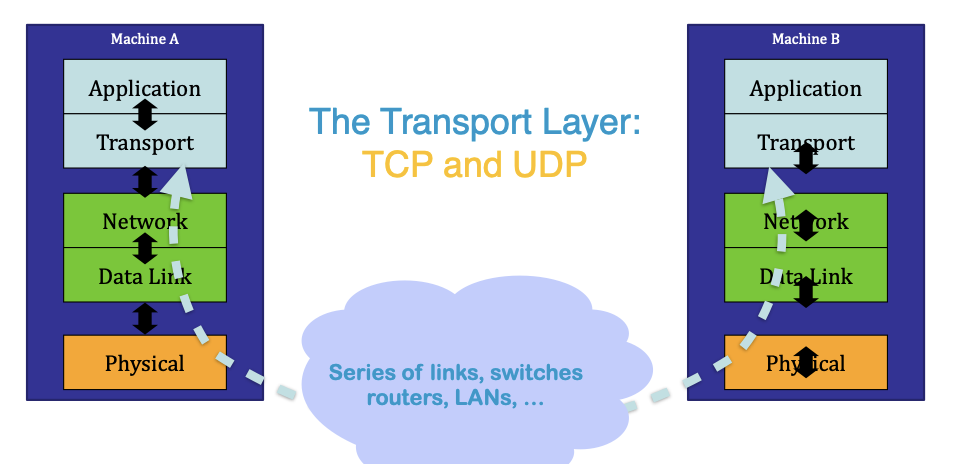
\includegraphics[width=0.8\textwidth]{transport-layer}
    \label{fig:LABEL}
\end{figure}

\section*{Contents}

1. UDP \\
2. TCP Basics: Sliding Window and Flow Control \\
3. TCP Connections and Sockets \\
4. More TCP Bells and Whistles \\
5. Secure Transport \\
6. Where should packet losses be repaired ?

\section*{Reminder from 1st lecture: Transport layer services}
\begin{minipage}{0.5\textwidth}
\begin{itemize}
	\item Network + Data link + Physical layer carry packets end-toend
	\item packets may be \textcolor{red}{lost} due to:
		\begin{itemize}
			\item errors at the physical layer
			\item buffer-overflow events at routers/switches
		\end{itemize}
	\item or \textcolor{red}{reordered} due to:
		\begin{itemize}
			\item following different paths to destination
		\end{itemize}
\end{itemize}

\end{minipage}
\begin{minipage}{0.5\textwidth}
\begin{itemize}
	\item Transport layer
		\begin{itemize}
			\item makes networks services available to pgraoms
			\item is in end-systems only, \textcolor{red}{not} in routers' data plane (i.e. not at forwarding level)
			\item may handle packet loss/reordering or not
				\begin{itemize}
					\item UDP \textcolor{red}{not reliable} transfer, takes no action
					\item TCP \textcolor{blue}{reliable, in-order} transfer by using sophisticated mechanisms
				\end{itemize}
		\end{itemize}
\end{itemize}
\end{minipage}

\begin{tcolorbox}[
  colback=gray!15,     % background color
  colframe=black!50,    % border color
  boxrule=1pt,       % border thickness
  arc=3mm,             % rounded corners
  left=4mm, right=4mm, top=2mm, bottom=2mm % padding
]
\textbf{What is the definition of a "server" in networks?}

\vspace{0.3cm}

A. A machine that hosts resources to be used in the web \\
B. A computer with high CPU performance \\
C. A computer with large data storage \\
D. The role of a program \\
E. The role of a program that allows users to access large amount of resources \\
F. None of the above \\
G. I don't know \\

\textbf{Answer:} D. \\
Formally, a server is a role at the transport layer, where the program waits for requests to come. In contrast, a client initiates communication to a server. \textbf{Port forwarding} comes from the need of allowing the client to start the connection. 
\end{tcolorbox}

\section*{Reminder from 1st lecture: Port Numbers}

\begin{itemize}
	\item Assigned by OS to identify processes within a host
 	\item servers' port numbers must be \textcolor{blue}{well-known} to clients (e.g., 53 for DNS, 80 for HTTP, 443 for HTTPS)
	\item src and dest port numbers are \textcolor{red}{inside transport-layer header}
\end{itemize}

% Quick centered image
\begin{figure}[H]
    \centering
    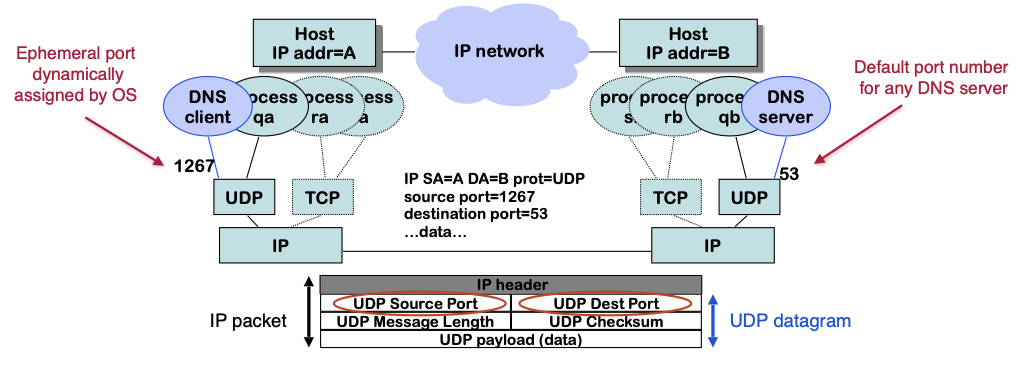
\includegraphics[width=1\textwidth]{ports}
    \label{fig:LABEL}
\end{figure}

\section*{1. UDP: message-oriented and unreliable}
\begin{itemize}
	\item UDP delivers either the exact message (a.k.a. "datagram") or nothing
	\item Each messages $\leq$ 65535 bytes (32 bits sequences)
	\item If a message is too large to fit into a single IP packet (i.e. larger than MTU), then IP layer \textcolor{blue}{fragments} it:
		\begin{itemize}
			\item not visible to the transport layer
			\item at source's IP layer, metadata about fragments is added to IP header
			\item if a fragment/piece is lost, then the entire message is lost
		\end{itemize}
	\item Application layer must handle \textcolor{red}{out of order} or \textcolor{red}{lost} messages, if needed
		\begin{itemize}
			\item e.g., DNS client resends DNS query if no response is received
		\end{itemize}
\end{itemize}

\section*{How is UDP implement in practice?}

Via \textcolor{red}{sockets} = programming interfaces
\begin{itemize}
	\begin{itemize}
		\item (in Unix) for read/write: sockets $\approx$ files
	\end{itemize}
 	\item \verb|socket(socket.AF_INET, ...)| resp. \verb|socket(socket.AF_INET6, ...)| creates and IPv4 (resp. IPv6) socket, returns an ID (= file descriptor)
	\item bind() associates an IP address + port number with a socket, can be skipped for the client
		\begin{itemize}
			\item \textcolor{blue}{Port = 0} $Rightarrow$ any available port
			\item  \textcolor{blue}{IP address = 0} $\Rightarrow$ all host's IP addresses
		\end{itemize}
	\item sendto() specifies: dest IP addresses, dest port number, and the message to send
	\item recvfrom() blocks until a message is received for this port number; it returns: src IP address, src port number and the message.
\end{itemize}

% Quick centered image
\begin{figure}[H]
    \centering
    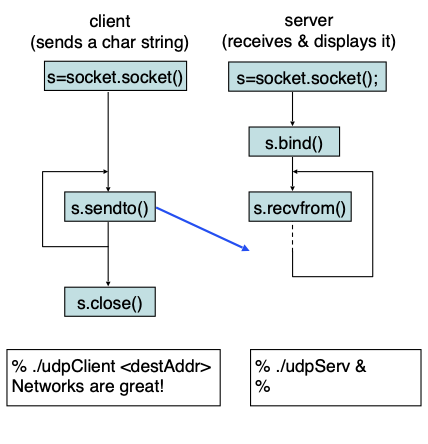
\includegraphics[width=0.6\textwidth]{sockets}
    \label{fig:LABEL}
\end{figure}

\section*{What socket to open? IPv4 or IPv6?}
\begin{itemize}
	\item Transport layer is not affected by the choice of IP (no UDPv6, not TCPv6)
	\item But, an application must choose IPv4 or IPv6, or better support both
\end{itemize}

\textcolor{red}{How?} Use \verb|socker.getaddrinfo()| to let the DNS give you whatever is available

\section*{IPv6 sockets can be \textcolor{red}{dual-stack}}

= bound to both IPv6 and IPv4 addresses of the local host 

= receive packets from IPv6 and/or IPv4 correspondents

\textcolor{red}{How?} The correspondents' IPv4 addresses are mapped to IPv6 addresses
\begin{itemize}
	\begin{itemize}
		\item using the \textcolor{red}{IPv4-mapped IPv5 address} format
		\item i.e., by appending the IPv4 address to prefix \verb|::ffff:0:0/96|
		% Quick centered image
		\begin{figure}[H]
		    \centering
		    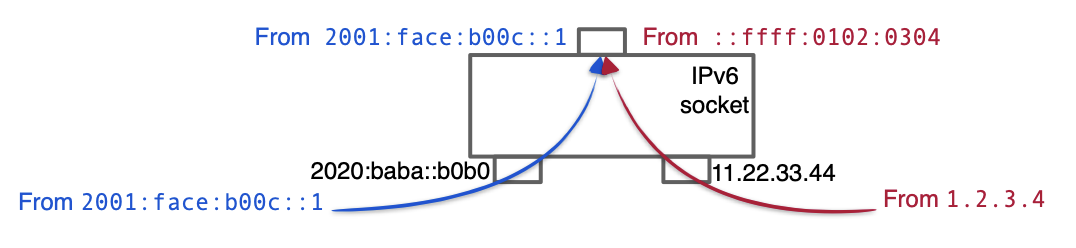
\includegraphics[width=0.8\textwidth]{ipv6-dual-stack}
		    \label{fig:LABEL}
		\end{figure}
	\end{itemize}
\end{itemize}
\begin{itemize}
	\item Default in Linux, must be enabled for every socket (with \verb|setsockopt| in Windows.
	\item An IPv4 socket \textcolor{blue}{cannot} be dual-stack. Why?
		\begin{itemize}
			\item That's because the IPv6 address space is munch longer in bits than the one from IPv4. Hence, an IPv4 socket cannot receive data from an IPv6 source address.
		\end{itemize}
\end{itemize}

\section*{How does the Operating System view UDP?}

UDP datagrams are delivered to sockets based on \textcolor{blue}{\textit{dest IP address}} and \textcolor{blue}{\textit{port number}}.
% Quick centered image
\begin{figure}[H]
    \centering
    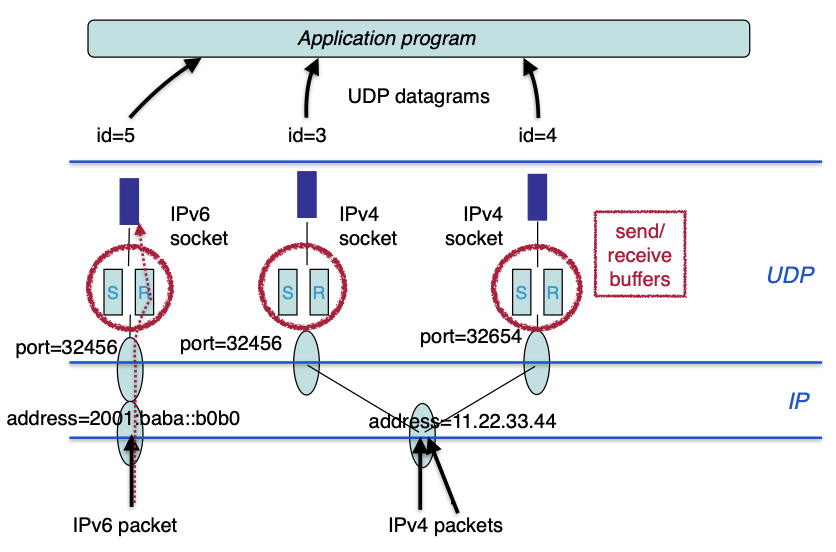
\includegraphics[width=0.8\textwidth]{os-udp}
    \label{fig:LABEL}
\end{figure}
\textbf{Note}: buffers can overflow! Receiver buffer is needed to assemble messages, sender buffer is necessary for congestion (for example WiFI carrier waits the channel to be free)

\section*{With a dual-stack IPv6 socket?}

\textbf{Socket 5} is bound to any local address, which includes IPv6 and IPv4 addresses, and to port 32456
% Quick centered image
\begin{figure}[H]
    \centering
    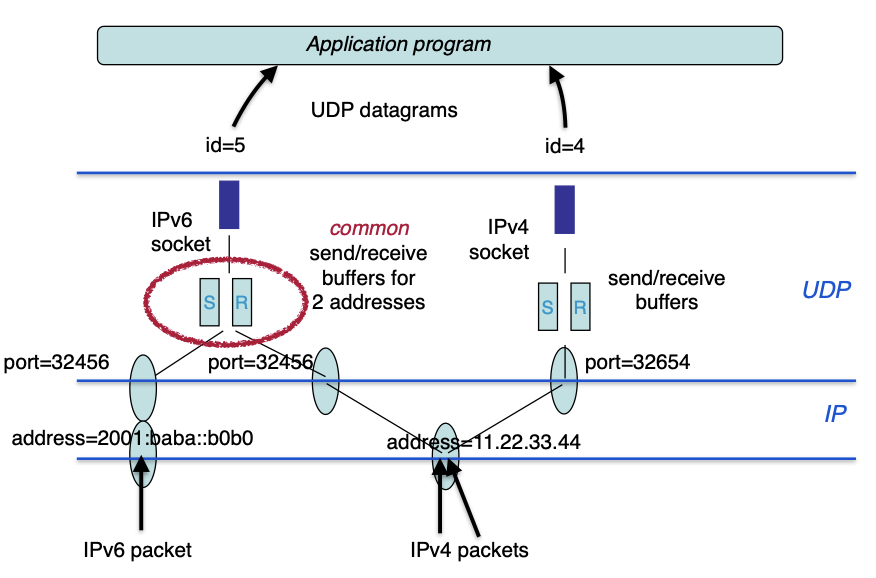
\includegraphics[width=0.8\textwidth]{os-dual-stack}
    \label{fig:LABEL}
\end{figure}

\begin{tcolorbox}[
  colback=gray!15,     % background color
  colframe=black!50,    % border color
  boxrule=1pt,       % border thickness
  arc=3mm,             % rounded corners
  left=4mm, right=4mm, top=2mm, bottom=2mm % padding
]
\textbf{User's browser sends DNS query to DNS server, over UDP. What happens if query or answer is lost?}

\vspace{0.3cm}

A. Name resolver in browser waits for timeout, if no answer received before timeout, sends again \\
B. Messages cannot be lost because UDP assures message integrity \\
C. UDP detects the loss and retransmits \\
D. I don't know \\

\textbf{Answer}: A
\end{tcolorbox}
\section*{Recap - UDP}

On the sending side: OS sends the UDP messages ASAP, but also uses a buffer to store data if interface is busy. OS may algo fragment the message if needed.

On the receiving side: OS re-assembles IP fragments of UDP message (if needed) and keeps the message in received buffer ready to be read. The message is: 
\begin{itemize}
	\item "\textcolor{blue}{\textit{consumed}}" when application reads
	\item or "\textcolor{blue}{\textit{dropped}}" because of an overflow event
\end{itemize}

A socket is bound to \textcolor{red}{a single port} and \textcolor{red}{one or multiple IP addresses} of the local host
\section*{2. TCP offers reliable, in-order delivery}

\textcolor{red}{What?}
\begin{itemize}
	\item TCP guarantees that all data is delivered \textcolor{red}{in order} and \textcolor{red}{without loss}, unless the connection is broken
\end{itemize}

\textcolor{red}{How?}
\begin{itemize}
	\item \textcolor{red}{Detects} reordering and loss, via sophisticated mechanisms:
		\begin{itemize}
			\item \textcolor{blue}{per-byte sequences numbers} 
			\item a connection-setup phase for the sender/receiver to \textcolor{blue}{synchronize} their sequence numbs
			\item \textcolor{blue}{acknowledgements}; if loss is detected, TCP retransmits
		\end{itemize}
	\item further optimizations, e.g.: 
		\begin{itemize}
			\item \textcolor{blue}{flow control} avoids buffer at the receiver
			\item TCP knows the allowable maximum segment size (\textcolor{blue}{MSS}) and segments data accordingly $\Rightarrow$ avoids fragmentation at the IP layer
		\end{itemize}
\end{itemize}

\subsection*{TCP Basic Operation 1: SEQ and ACK}

\begin{minipage}{0.4\textwidth}
\begin{itemize}
	\item The applications at A sends that in blocks of 500 bytes at a slow pace. So, TCP initially sends 500-byte segments
	\item However, the MSS in this example is 1000 bytes. So, TCP may also merge 2 blocks of data in one segment if this data happens to be available at the send buffer of the socket
	\item B returns an acknowledgement in the ACK field. The ACK Field is \textcolor{red}{\textit{cumulative}}, so ACK 85001 means: B is acknowledging all byes up to (excluding) number 8501.
	\item The out-of-order received data is kept in the buffer until all data is received correctly - this is not visible to the application. 
\end{itemize}

\end{minipage}
\hfill
\begin{minipage}{0.7\textwidth}
\centering
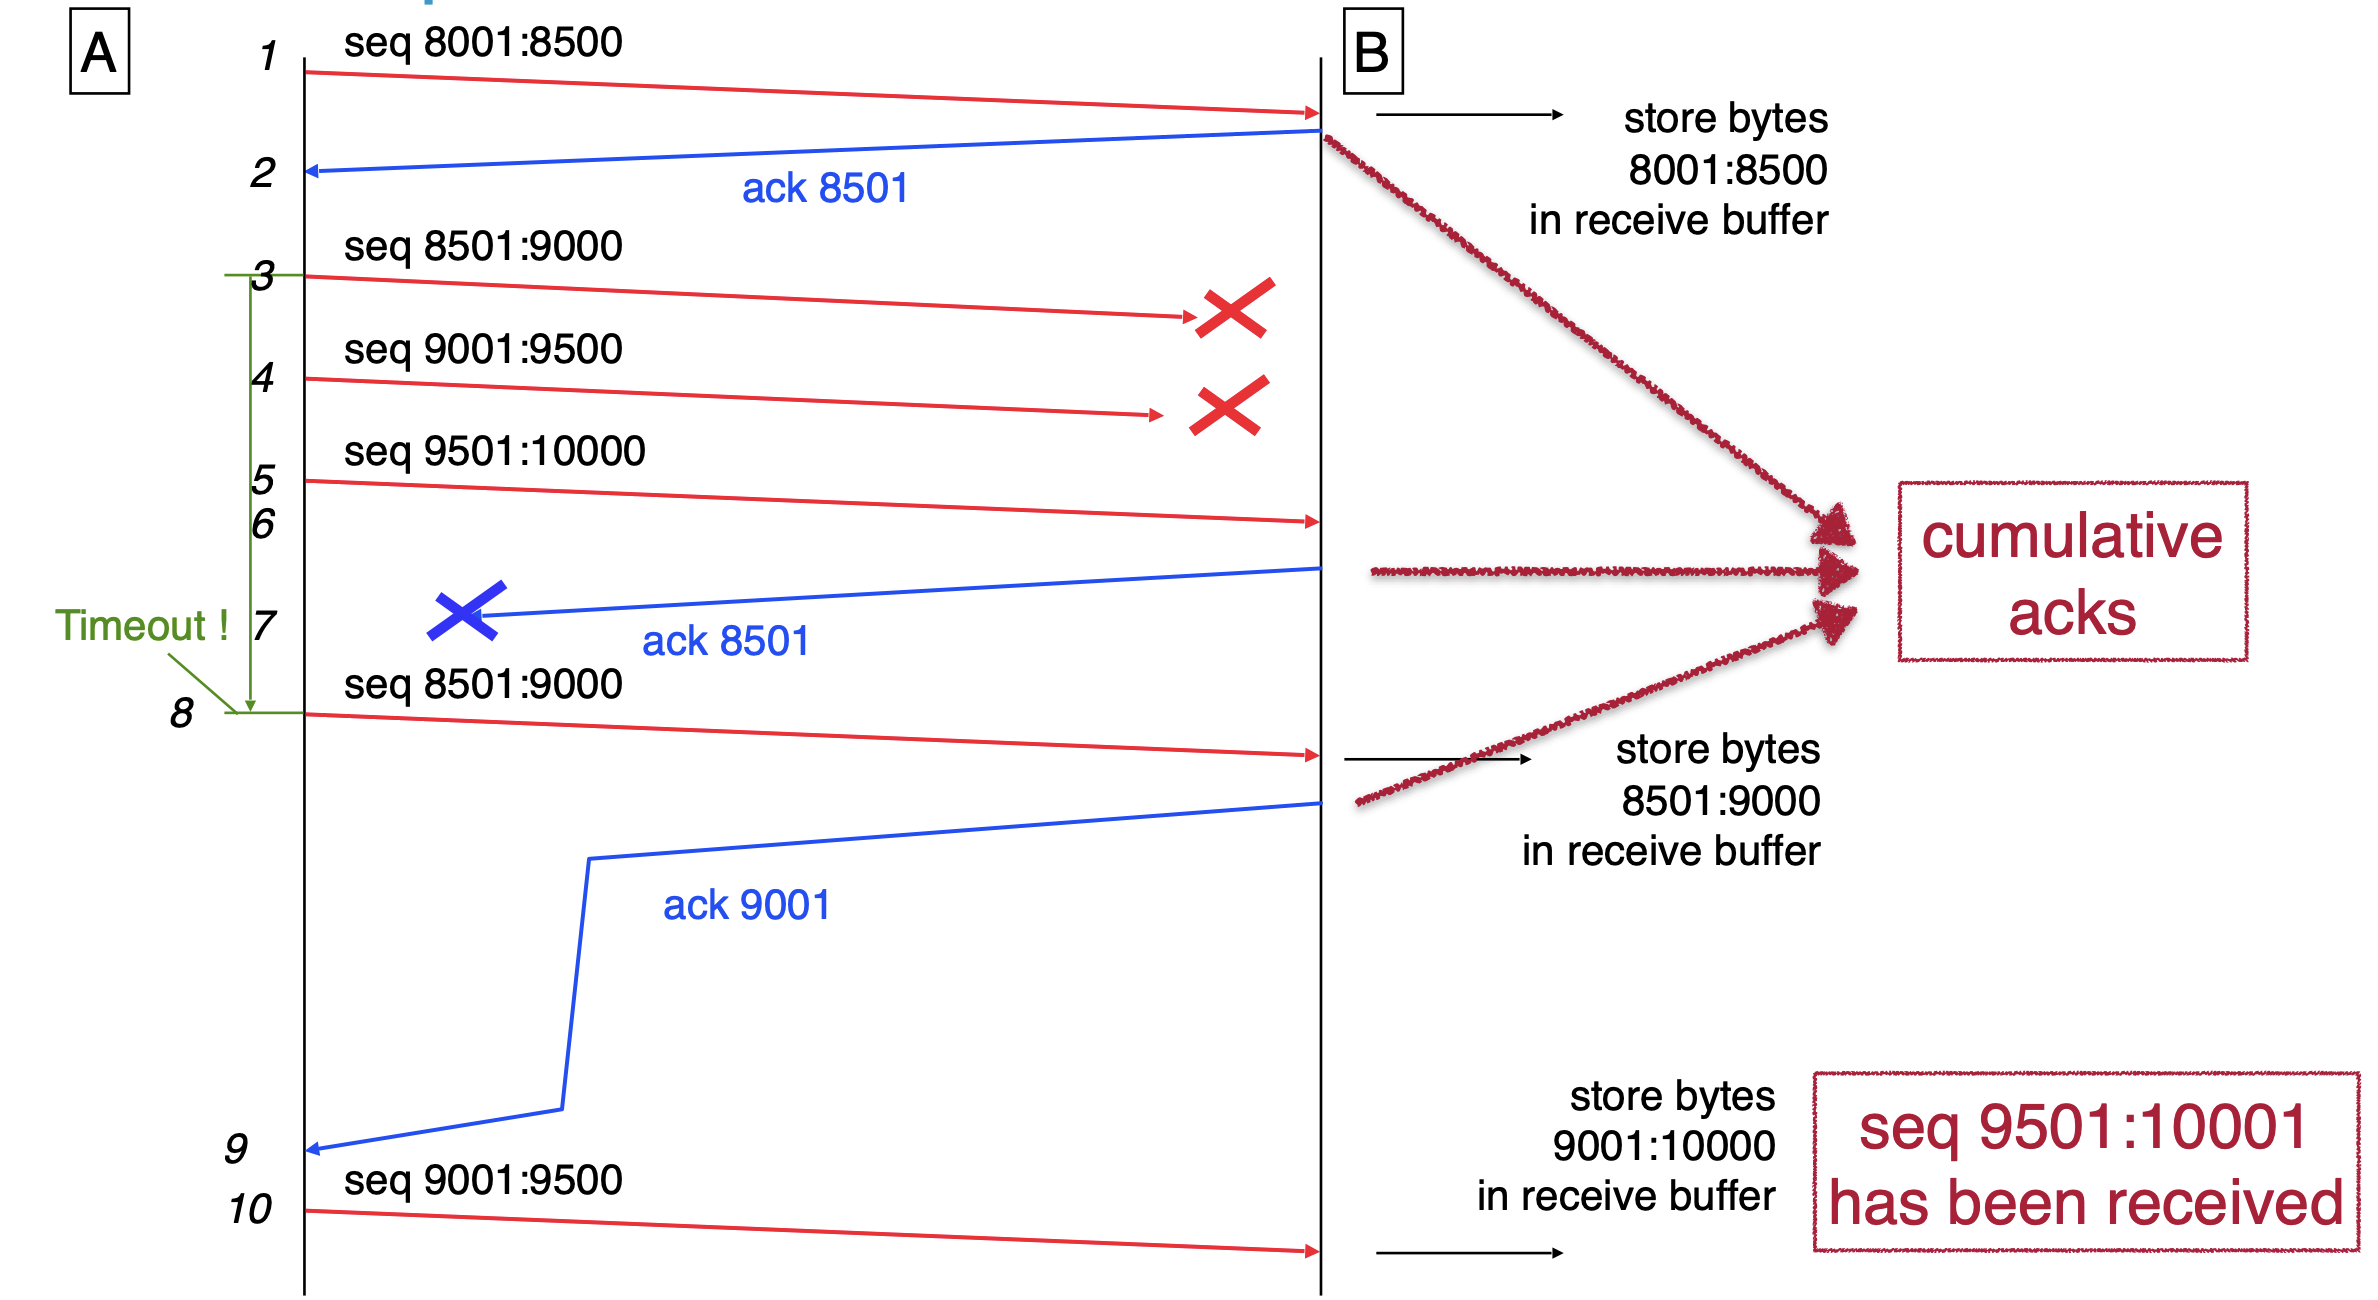
\includegraphics[width=\linewidth]{tcp1}
\end{minipage}

\subsection*{TCP Basic Operations 2: SACK and optimized segmentation (if possible)}

\begin{minipage}{0.4\textwidth}
In addition to the ACK field, most TCP implementation also use the SACK field (\textit{\textcolor{red}{Selective Acknowledgement}}).
\begin{itemize}
	\item At line 7, B acknowledges all bytes up to 8501 and in the range 9501:10000. Since the set of acknowledged byes is not contiguous, the SACK option is used. It contains up to 3 blocks that are acknowledged in addition to the range described by the ACK field
	\item At line 8, A detects that the bytes 8501:9500 were lost and re-sends them ASAP without waiting for a timeout. Since the MSS is 1000 bytes, only one packet it sent (optimized segmentation). 
	\item When receiving packet 8, B can deliver bytes 9001:10000 because packet 5 was received and kept in the receive buffer.
\end{itemize}
\end{minipage}
\hfill
\begin{minipage}{0.7\textwidth}
\centering
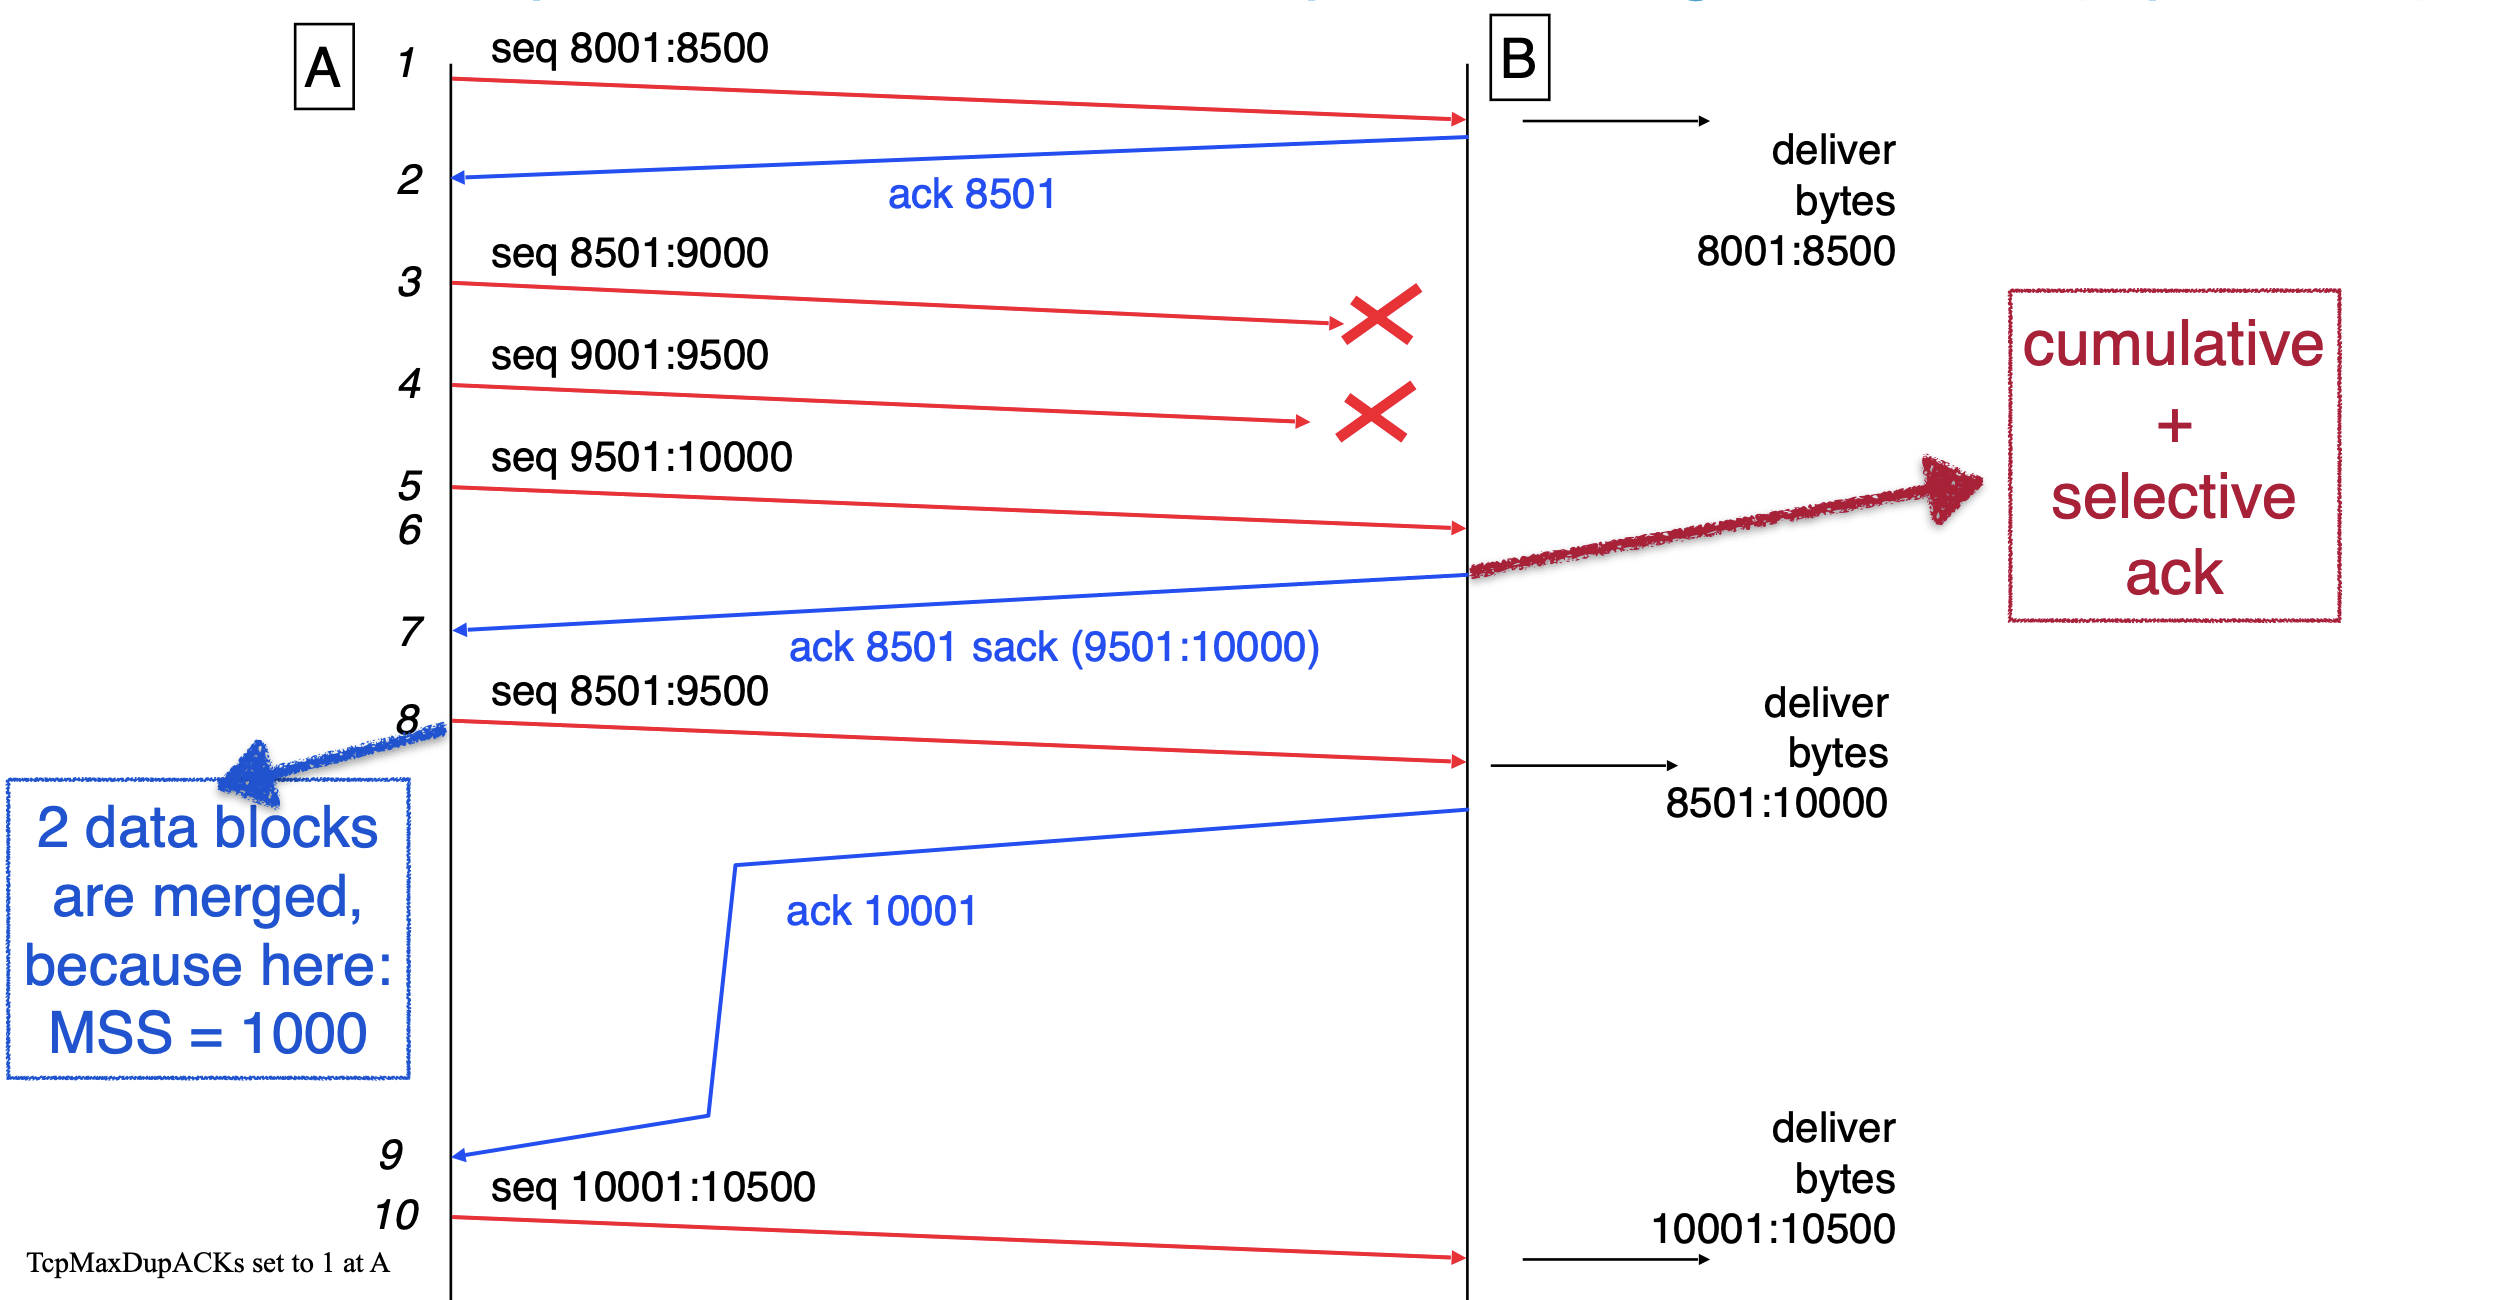
\includegraphics[width=\linewidth]{tcp2}
\end{minipage}

\subsection*{Receive Buffer}

TCP receiver uses a \textit{\textbf{receive buffer}} = \textcolor{red}{\textit{re-sequencing}} buffer to store incoming packets before delivering them to the application. 

\textcolor{red}{\textit{Why}} invented?
\begin{itemize}
	\item Application may not be ready to consume/read data
	\item Packets may need re-sequencing; out-of-order data is stored but is \textcolor{red}{\textit{not visible}} to application
\end{itemize}
% Quick centered image
\begin{figure}[H]
    \centering
    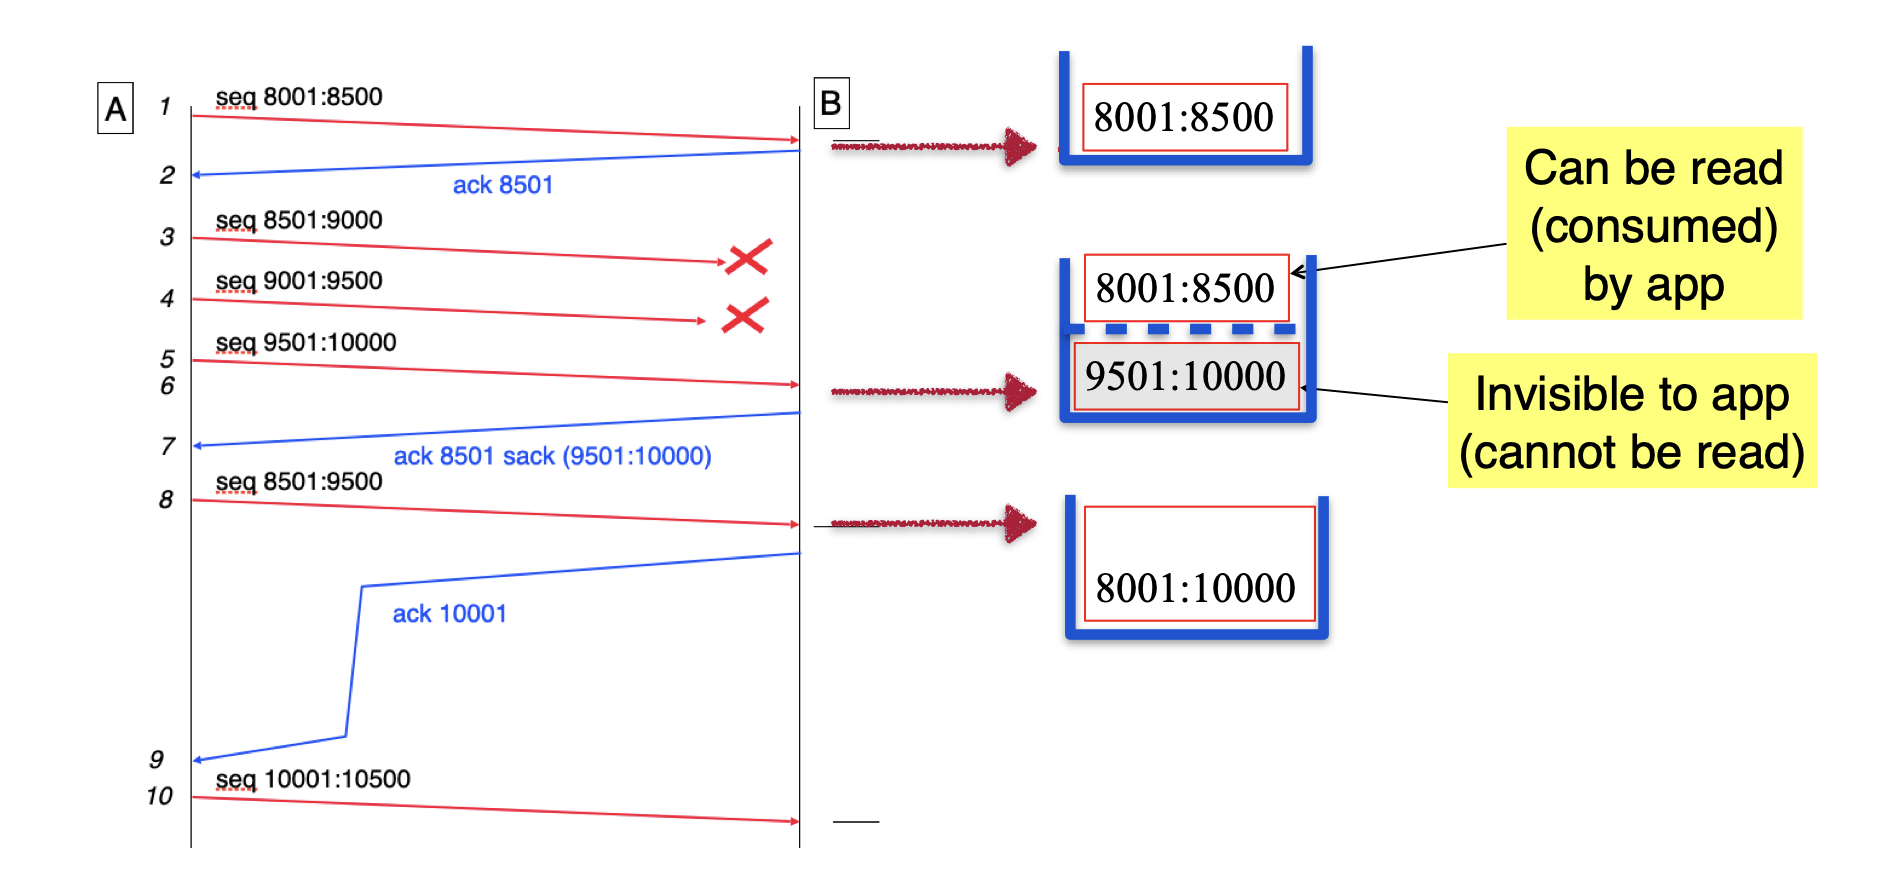
\includegraphics[width=0.9\textwidth]{tcp3}
    \label{fig:LABEL}
\end{figure}

\subsection*{TCP uses a sliding window}

\begin{minipage}{0.5\textwidth}
\textcolor{red}{\textit{Why?}} \\
\begin{itemize}
	\item Out-of-order packets may trigger buffer \textcolor{red}{\textit{overflows}} \\
	\item The sliding window \textcolor{blue}{\textit{limits}} the number of data

\end{itemize}
\end{minipage}
\hfill
\begin{minipage}{0.3\textwidth}
\centering
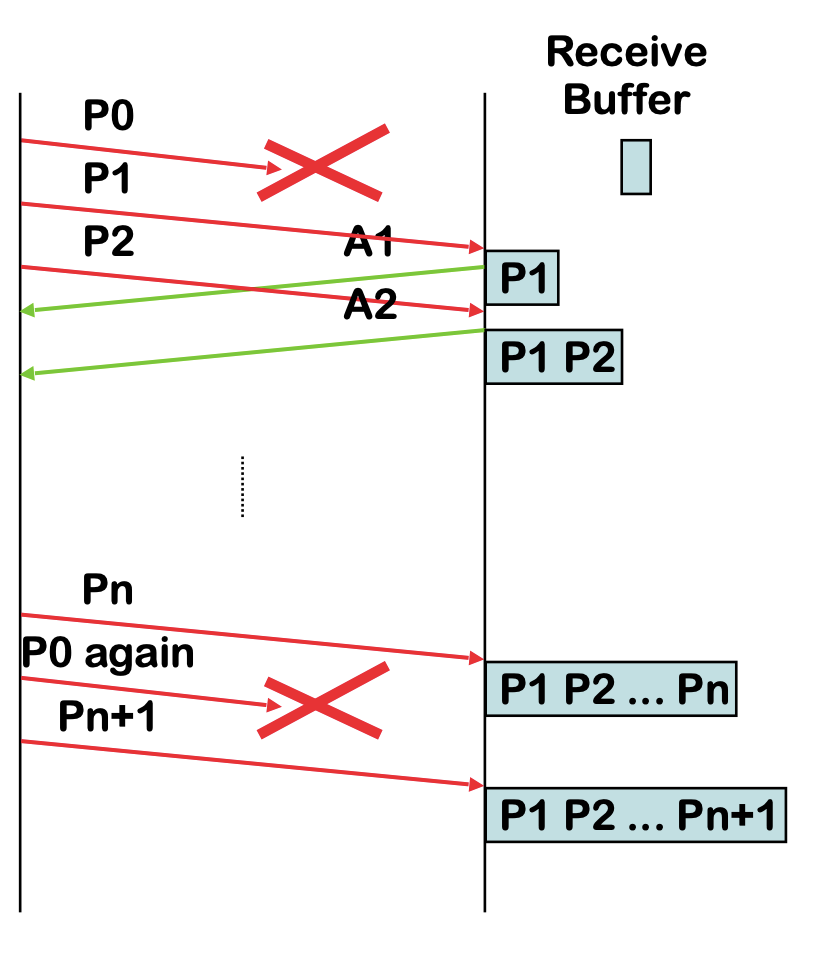
\includegraphics[width=\linewidth]{tcp4}
\end{minipage}

\subsection*{How does the sliding window work?}

\begin{minipage}{0.4\textwidth}
\begin{itemize}
	\item Suppose: window size = 4000B; each segment = 1000B. \\
	\item Only seq numbers within the window can be sent (and are sent if enough data exist in the socket) \\
	\item \texttt{lower window edge = smallest non-ack'ed sequence number} \\
	\item \texttt{upper window edge = lower\_edge + window\_size} \\
\end{itemize}

\end{minipage}
\hfill
\begin{minipage}{0.6\textwidth}
\centering
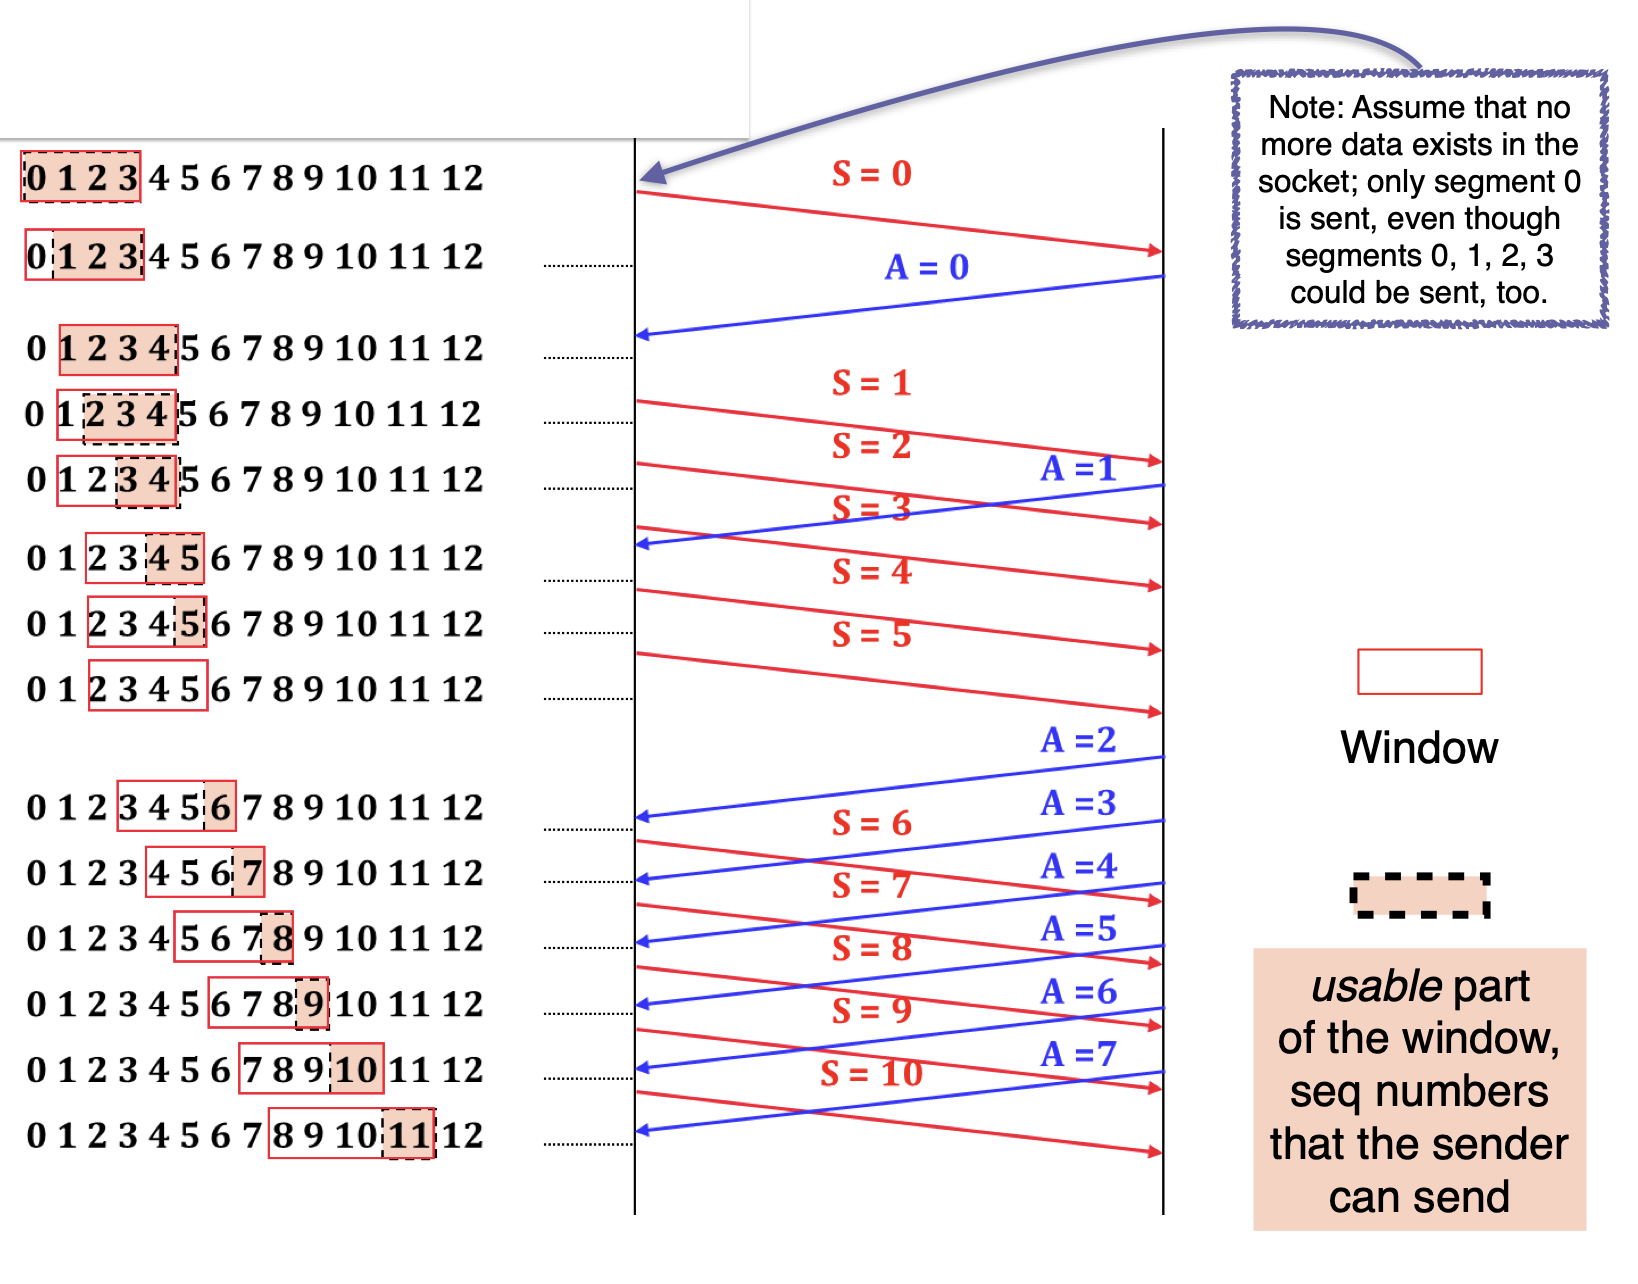
\includegraphics[width=\linewidth]{tcp5}
\end{minipage}

\end{document}	
